 \documentclass{report}
 
\usepackage[utf8]{inputenc} 
\usepackage[T1]{fontenc}      
\usepackage[top=2.0cm, bottom=3cm, left=3.0cm, right=3.0cm]{geometry}
\usepackage{graphicx}
\usepackage{wrapfig}
\usepackage{amsmath,esint }
\usepackage{amssymb}
\graphicspath{{figures/}{../figures}}

\newcommand*\dif{\mathop{}\!\mathrm{d}}
\newcommand*\diver{\mathop{}\!\mathrm{div}}
\newcommand*\grad{\mathop{}\!\mathrm{grad}}

\begin{document}

\section*{Sillage d'un avion}

On considère le vol d'un avion de chasse $A$ se déplaçant dans le sens des $x$ croissants, à une vitesse $v$ sur une droite horizontale $(y=0,z=h)$ alors qu'un observateur est situé au point $O(0,0,0)$. L'avion émet un signal sonore de période $T$. On note $\theta=(\vec{Ox},\vec{OA})$ l'inclinaison par rapport à l'horizontale de la direction observateur-avion. Cet angle est supposé varier peu pendant une période $T$.

\begin{itemize}

	\item[$\circ$] L'air a une masse volumique au repos $\rho_0$ et une compressibilité $\chi_s$. Retrouver l'équation d'Alembert caractérisant la propagation des ondes sonores dans l'air, en explicitant la vitesse de propagation $c$ des ondes.

\end{itemize}

On suppose dans un premier temps que l'avion se déplace à une vitesse subsonique, c'est-à-dire $v<c$.

\begin{itemize}

	\item[$\star$] On appelle $t_1$ et $t_2$ deux moments successifs où le signal sonore est émis (donc $t_2-t_1=T)$, et $t'_1$ et $t'_2$ les deux moments successifs où ces signaux sont reçus par l'observateur. Exprimer la période $T'=t'_2-t'_1$ en fonction de $h$, $c$, $\theta_1=\theta(t_1)$ et $\theta_2=\theta(t_2)$. 
	
	\item[$\star$] En déduire est la période $T'$ du signal perçu par l'observateur en fonction de $\theta$. Comment s'appelle ce phénomène ?

\end{itemize}

On suppose désormais que l'avion se déplace à une vitesse supersonique, c'est-à-dire $v>c$.

\begin{itemize}

	\item[$\diamond$] Le son émis par l'avion à l'instant $t$ est perçu par l'observateur à l'instant $t'=f(t)$. Déterminer la fonction $f$ si l'avion passe à l'instant $t=0$ à la verticale de l'observateur. En s'appuyant sur les asymptôtes de $t'$ dans les cas $t\longrightarrow\pm\infty$, représenter graphiquement $f(t)$.
	
	\item[$\diamond$]  Pourquoi le son perçu est-il particulièrement intense si $\dif t'/\dif t=0$ ? Comment s'appelle ce phénomène ? 
	
	\item[$\diamond$]  On donne $h=1000$m ; $v=500$m.s$^{-1}$ ; $c=340$m.s$^{-1}$. On note $t'_0$ l'instant auquel le bang est perçu par l'observateur et $t_0$ l'instant auquel les sons perçus à l'instant $t'_0$ ont été émis par l'avion. Déterminer $t_0$, $t'_0$ et les positions de l'avion à $t_0$ et $t'_0$. 
	
	\item[$\diamond$] L'observateur entend-il l'avion avant d'entendre le bang ? Quelle est la durée $\Delta t$ d'émission des sons perçus entre $t'_0$ et $t'_0+\Delta t'$ (on pourra effectuer une développement limité de $f(t)$). Calculer $\Delta t$ pour $\Delta t'=0.1$s et commenter.
	
	\item[$\diamond$] Quelle est la région de l'espace qui peut être atteinte à un instant donné par une onde sonore provenant de l'avion ?
	
	\item[$\diamond$] Estimer la vitesse de l'avion en photo ci-dessous.  

\end{itemize}

\begin{figure}[h!]
\centering
		\includegraphics[scale=0.10]{avion.jpg}
\end{figure}

\newpage

\section*{Pavillon acoustique}

\subsubsection{Propagation du son dans l'air libre}

L'air a une masse volumique au repos $\rho_0$ et une compressibilité $\chi_s$. Les vibrations des ondes sonores sont caractérisées par des variations locales du champ de pression $p$, de masse volumique $\mu$ et de vitesse $v$. 

\begin{itemize}

	\item[$\circ$] Qu'est-ce que l'approximation accoustique ? On supposera qu'elle est toujours vérifée par la suite.

	\item[$\circ$]  Retrouver l'équation d'Alembert caractérisant la propagation des ondes sonores dans l'air, en explicitant la vitesse de propagation $c$ des ondes.

\end{itemize}

\subsubsection{Propagation du son dans un pavillon}

On s'intéresse désormais à un pavillon acoustique, de symétrie de révolution autour de l'axe $Ox$, a une section $S(x)$ à l'abscisse $x$, contenant de l'air de masse volumique $\rho_0$ et de compressibilité $\chi_s$. Une onde s'y propage suivant $Ox$, mais contrairement à de l'air libre, les parois du pavillon imposent une contrainte sur la propagation du son. On note $p(x,t)$ la surpression acoustique et $\Psi(x,t)$ le déplacement longitudinal de la tranche de fluide en $x$ à l'instant $t$. 

\begin{figure}[h!]
\centering
		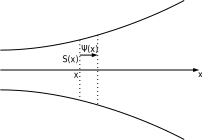
\includegraphics[scale=1.2]{onde_pavillon.pdf}
\end{figure}

\begin{itemize}

\item[$\diamondsuit$] En reliant la compressibilité $\chi_s=-\frac{1}{V}\frac{\partial V}{\partial P}$ à la surpression $p(x,t)$ et au déplacement $\Psi(x,t)$, démontrer la relation suivante :
\begin{align*}
	p(x,t) = -\frac{1}{\chi_s}\left(\frac{\partial \Psi}{\partial x}+\Psi(x,t)\frac{\partial }{\partial x}\left[\ln S(x) \right]  \right)
\end{align*}

\item[$\diamondsuit$] En faisant un bilan de quantité de mouvement sur un fluide, en déduire une relation similaire à une équation "d'onde" portant sur $\Psi(x,t)$.

\end{itemize}

Le pavillon a une allure exponentielle : $S(x)=S_0\exp(ax)$. On suppose que l'onde est une onde plane, progressive et monochromatique : $p(x,t)=p_0\exp\left(j[\omega t-kx] \right)$. On notera la vitesse de déplacement $v(x,t)=\partial\Psi/\partial t$.

\begin{itemize}

\item[$\diamondsuit$] Montrer que l'équation "d'onde" vérifiée par $\Psi(x,t)$ est aussi vérifiée par $p(x,t)$. On pourra donc injecter la solution en $p(x,t)$ proposée dans l'équation "d'onde".

\item[$\diamondsuit$]  Trouver une équation entre $k$ et $\omega$. En déduire l'expression de $k$ en fonction de $\omega$. Distinguer deux cas.

\item[$\diamondsuit$] Montrer qu'il ne peut pas y avoir de propagation de l'onde sonore en dessous d'une certaine pulsation de coupure $\omega_c$.

\item[$\diamondsuit$] Donner les expression de $v(x,t)$, $p(x,t)$, puis celle de l'énergie acoustique $\varepsilon(x,t)$ et du vecteur de densité de dourant d'énergie sonore $R_s(x,t)$.

\end{itemize}

\newpage

\section*{Impédance acoustique}

On considère une onde acoustique se propageant selon les $x$ croissants dans un milieu 1 ($x<0$) et atteignant le milieu 2 ($x>0$) en $x=0$. Les milieux 1 et 2 dans lesquels se propagent une onde sonore sont caractérisés respectivement par une masse volumique $\rho_1$ et $\rho_2$ et une célérité des ondes acoustiques $c_1$ et $c_2$. 

\subsubsection*{Échographie}

\begin{itemize}
	
	\item[$\spadesuit$] Retrouver l'équation d'Alembert vérifiée par la surpression $p(x,t)$ et la vitesse $v(x,t)$ dans un milieu homogène. Quelles sont les solutions générales dans ce cas unidimensionnel ? 

\end{itemize}	
	
On suppose que les champs de vitesse et de surpression sont des ondes planes progressives monochromatique et s'écrivent (l'indice $j$ représentant le milieu 1 ou 2) :
\begin{align*}
	\vec{v}_j(x,t)&=v_{0,j}\exp\left[i(k_jx\pm \omega t) \right] \vec{e}_x \\
	p_j(x,t)&=p_{0,j}\exp\left[i(k_jx\pm \omega t) \right]
\end{align*}

\begin{itemize}
	
	\item[$\spadesuit$] Quelle relation vérifient $k_j$ et $\omega$ ? En déduire une autre relation entre l'amplitude des champs de vitesse $v_{0,j}$ et de pression $p_{0,j}$. On introduira la notion d'impédance acoustique.
	
	\item[$\spadesuit$] Écrire les relations que vérifient la vitesse et la surpression à l'interface en $x=0$. Justifier. 
	
	\item[$\spadesuit$] Une onde incidente $v_{0,i}\exp\left[i(k_1x- \omega t) \right] \vec{e}_x$  arrive sur l'interface depuis le milieu 1. Pourquoi a t-on nécessairement l'apparition d'une onde réfléchie et d'une onde transmise à l'interface si les milieux 1 et 2 ne sont pas les mêmes ?
	
	\item[$\spadesuit$] Exprimer les coefficients de réflexion en vitesse $r_v=v_{0,r}/v_{0,i}$ et de transmission $t_v=v_{0,t}/v_{0,i}$, puis les coefficients de réflexion en pression $r_v=p_{0,r}/p_{0,i}$ et de transmission $t_v=p_{0,t}/p_{0,i}$
	
	\item[$\spadesuit$]	 En déduire les coefficients de réflexion $R$ et de transmission $T$ en intensité. 
	
	\item[$\spadesuit$] Pourquoi dont-on mettre un gel sur entre la sonde et le corps durant une échographie ? 
		
\end{itemize}

\subsubsection*{Isolation phonique}

On suppose qu'il y a désormais une paroi de masse surfacique $\mu$ à l'interface entre les deux milieux, qui sont supposées être identiques ($\rho_1=\rho_2$ et $c_1=c_2$). Cette paroi se meut librement et sans frottement. 

\begin{itemize}
	
	\item[$\clubsuit$] Que deviennent les relations de passage précédentes ? En déduire le coefficient de transmission en vitesse $t_v$ dans ce cas-là. 
	
	\item[$\clubsuit$] Calculer $T=\mid t\mid^2$ et tracer l'allure de la courbe $G_{db}=20\log\left[T(\omega) \right]$ en fonction de $\log(\omega)$. Quelle est la fréquence de coupure ?
	
	\item[$\clubsuit$] Expliquer pourquoi les sons graves se transmettent mieux à travers les parois (un mur par exemple) que les sons aigus.
	
\end{itemize}

\newpage

\section*{Silencieux de ligne d'échappement}

On étudie la réflexion et la transmission d'ondes sonores planes dans un fluide homogène au niveau d'un raccordement  de deux conduites de sections $S_1$ et $S_2$. 

\begin{itemize}
	
	\item[$\spadesuit$] Retrouver l'équation d'Alembert vérifiée par la surpression $p(x,t)$ et la vitesse $v(x,t)$ dans chaque milieu homogène 1 ou 2. Quelles sont les solutions générales à cette équation ? 

	\item[$\spadesuit$] Qu'appelle t-on les ondes planes progressives monochromatiques ? On suppose que ce modèle d'onde permet de décrire les champs de surpression $p(x,t)$ et la vitesse $v(x,t)$ dans notre cas. Proposer une expression pour ces champs dans le milieu 1 et 2.
	
	\item[$\spadesuit$] Écrire les relations que vérifient la vitesse et la surpression à l'interface en $x=0$. Justifier.
	
	\item[$\spadesuit$] Que se passe t-il lorsqu'une onde plane progressive arrive de par la gauche sur l'interface $1\longrightarrow2$ pour que ces relations soient vérifiées ?
	
	\item[$\spadesuit$] En déduire les coefficients de réflexion $r=v_r/v_i$ et de transmission $t=v_t/v_i$, où $v_i$, $v_r$ et $v_t$ sont respectivement l'amplitude du champ de vitesse de l'onde incidente, réfléchie et transmise. Expliciter une impédance "acoustique" dont dépend les coefficients de réflexion et de transmission.
	
	\item[$\spadesuit$] Commenter les cas $S_2=\infty$ et $S_2=0$.

\end{itemize}

\end{document}
